\documentclass[a4paper]{article}
\usepackage{geometry}
\usepackage{graphicx}
\usepackage{natbib}
\usepackage{amsmath}
\usepackage{amssymb}
\usepackage{amsthm}
\usepackage{paralist}
\usepackage{epstopdf}
\usepackage{tabularx}
\usepackage{longtable}
\usepackage{multirow}
\usepackage{multicol}
\usepackage[hidelinks]{hyperref}
\usepackage{fancyvrb}
\usepackage{algorithm}
\usepackage{algorithmic}
\usepackage{float}
\usepackage{paralist}
\usepackage[svgname]{xcolor}
\usepackage{enumerate}
\usepackage{array}
\usepackage{times}
\usepackage{url}
\usepackage{fancyhdr}
\usepackage{comment}
\usepackage{environ}
\usepackage{times}
\usepackage{textcomp}
\usepackage{caption}


\urlstyle{rm}

\setlength\parindent{0pt} % Removes all indentation from paragraphs
\theoremstyle{definition}
\newtheorem{definition}{Definition}[]
\newtheorem{conjecture}{Conjecture}[]
\newtheorem{example}{Example}[]
\newtheorem{theorem}{Theorem}[]
\newtheorem{lemma}{Lemma}
\newtheorem{proposition}{Proposition}
\newtheorem{corollary}{Corollary}

\floatname{algorithm}{Procedure}
\renewcommand{\algorithmicrequire}{\textbf{Input:}}
\renewcommand{\algorithmicensure}{\textbf{Output:}}
\newcommand{\abs}[1]{\lvert#1\rvert}
\newcommand{\norm}[1]{\lVert#1\rVert}
\newcommand{\RR}{\mathbb{R}}
\newcommand{\CC}{\mathbb{C}}
\newcommand{\Nat}{\mathbb{N}}
\newcommand{\br}[1]{\{#1\}}
\DeclareMathOperator*{\argmin}{arg\,min}
\DeclareMathOperator*{\argmax}{arg\,max}
\renewcommand{\qedsymbol}{$\blacksquare$}

\definecolor{dkgreen}{rgb}{0,0.6,0}
\definecolor{gray}{rgb}{0.5,0.5,0.5}
\definecolor{mauve}{rgb}{0.58,0,0.82}

\newcommand{\Var}{\mathrm{Var}}
\newcommand{\Cov}{\mathrm{Cov}}

\newcommand{\vc}[1]{\boldsymbol{#1}}
\newcommand{\xv}{\vc{x}}
\newcommand{\Sigmav}{\vc{\Sigma}}
\newcommand{\alphav}{\vc{\alpha}}
\newcommand{\muv}{\vc{\mu}}

\newcommand{\red}[1]{\textcolor{red}{#1}}

\def\x{\mathbf x}
\def\y{\mathbf y}
\def\w{\mathbf w}
\def\v{\mathbf v}
\def\E{\mathbb E}
\def\V{\mathbb V}

% TO SHOW SOLUTIONS, include following (else comment out):
\newenvironment{soln}{
    \leavevmode\color{blue}\ignorespaces
}{}


\hypersetup{
%    colorlinks,
    linkcolor={red!50!black},
    citecolor={blue!50!black},
    urlcolor={blue!80!black}
}

\geometry{
  top=1in,            % <-- you want to adjust this
  inner=1in,
  outer=1in,
  bottom=1in,
  headheight=3em,       % <-- and this
  headsep=2em,          % <-- and this
  footskip=3em,
}


\pagestyle{fancyplain}
\lhead{\fancyplain{}{Homework 1}}
\rhead{\fancyplain{}{CS 760 Machine Learning}}
\cfoot{\thepage}

\title{\textsc{Homework 1}} % Title

%%% NOTE:  Replace 'NAME HERE' etc., and delete any "\red{}" wrappers (so it won't show up as red)

\author{
\red{$$AKASH SHARMA$$} \\
\red{$$9081731771$$}\\
} 

\date{}

\begin{document}

\maketitle 


\textbf{Instructions:} 
This is a background self-test on the type of math we will encounter in class. If you find many questions intimidating, we suggest you drop 760 and take it again in the future when you are more prepared.

Use this latex file as a template to develop your homework.
Submit your homework on time as a single pdf file to Canvas.
There is no need to submit the latex source or any code.
Please check Piazza for updates about the homework.


\section{Logistics [5 pts]}
Read the course webpage at \url{http://pages.cs.wisc.edu/~jerryzhu/cs760.html} and answer the following questions:
\begin{enumerate}

\item Where do we post announcements and clarifications?
\begin{soln}  
\\ Piazza
\end{soln}

%\item Where do we post announcements and clarifications?
%\\\textbf{Ans.} Piazza

\item What time of day (hour:minute) are all homeworks due?
\begin{soln} 
\\ 10:59 AM
\end{soln} 

\item Will late homework be accepted?
\begin{soln} 
\\ No, late homework will not be accepted.
\end{soln} 

\item Tom received the following scores on his 7 homeworks: 0, 59, 92, 95, 98, 100, 100.  According to the homework policies, what is Tom's final average homework score?
\begin{soln} 
\\ Lowest score 0 will be dropped from final average calculation. Final average is 90.67.
\end{soln} 

\item How can you discuss homework questions with fellow students while avoiding the impression of cheating?
\begin{soln} 
\\ We can discuss the homework approaches and techniques broadly with other fellow students. However, all examinations, programming assignments, and written homeworks must be written up individually. Also, for programming assignments the code must not be developed in groups, nor should code be shared. We need to make sure to work independently on all the problems and write our own final writeups.
\end{soln} 

\end{enumerate}

\section{Vectors and Matrices [2 pts]}
Consider the matrix $X$ and the vectors $\mathbf{y}$ and $\textbf{z}$ below:
$$
X = \begin{pmatrix}
6 & 7 \\ 8 & 9 \\
\end{pmatrix}
\qquad \mathbf{y} = \begin{pmatrix}
2 \\ 3
\end{pmatrix} \qquad \mathbf{z} = \begin{pmatrix}
7 \\ 6
\end{pmatrix}
$$
\begin{enumerate}
	\item 	Computer $\mathbf{y}^\top X \mathbf{z}$\\
	    \begin{soln} 
				
				$\mathbf{y}^{T} = \begin{pmatrix}
				2 & 3
				\end{pmatrix} $\\

				$\mathbf{y}^{T} X = \begin{pmatrix}
				36 & 41
				\end{pmatrix} $\\

	 $\mathbf{y}^\top X \mathbf{z} = 36*7 + 41*6 = 498 
	$\\	


	    \end{soln}

	\item 	Is $X$ invertible? If so, give the inverse, and if no, explain why not.\\
        \begin{soln}  
		
		Yes, X is Invertible as its determinant is non-zero. The determinant is: 6*9 – 7*8 = 54 – 56 = -2.
		Inverse of X is,
	
				   $$	
				    \begin{pmatrix} -4.5 & 3.5 \\ 4 & -3 \\\end{pmatrix}			
				  $$	
	 \end{soln}
\end{enumerate}


\section{Calculus [1 pts]}
\begin{enumerate}
	\item If $y = e^x + \tan(z)x^{6z} - \ln(\frac{7x + z}{x^{4}})$, what is the partial derivative of $y$ with respect to $x$?\\
	\begin{soln}  

		Partial derivative of the above expression is:  
		$$
		e^x + 6z\tan(z)x^{6z-1} + (4/x) – (7/(7x+z))
 		$$

	\end{soln}

\end{enumerate}




\section{Probability and Statistics [4 pts]}
Consider a sequence of data $S = (0, 1, 1, 0, 1, 1, 1)$ created by flipping a coin $x$ seven times, where 0 denotes that the coin turned up heads and 1 denotes that it turned up tails.
\begin{enumerate}
	\item 	What is the probability of observing this data, assuming it was generated by flipping a biased coin with $p(x=1) = 0.7$?
	    \begin{soln}  

			$p(x=1) = 0.7$
			$p(x=0) = 0.3$

			Probablility of observing this data =  0.3 * 0.7 * 0.7 * 0.3 * 0.7 * 0.7 * 0.7 = 0.0151263
	    \end{soln}

	\item 	Note that the probability of this data sample could be greater if the value of $p(x = 1)$ was not $0.7$, but instead some other value. What is the value that maximizes the probability of $S$? Please justify your answer.\\
	    \begin{soln}  

				Let  $p(x = 1) = t $, hence, the Probablility of S becomes:
				$ t^{5}*(1-t)^{2}.$
				\\Taking partial derivative to get the value of t to maximize the above, we get 
				$$
				 5*(1-t) = 2*t	
				$$
				\\Hence, $ t = p(x = 1) = 5/7 $
	   \end{soln}

	\item 	Consider the following joint probability table where both $A$ and $B$ are binary random variables: 
\begin{table}[htb]
\centering
	\begin{tabular}{ccc}\hline
	A & B & $P(A, B)$  \\\hline
	0 & 0 & 0.4 \\
	0 & 1 & 0.3 \\
	1 & 0 & 0.2 \\
	1 & 1 & 0.1 \\\hline
	\end{tabular}
\end{table}
\begin{enumerate}
	\item 	What is $P(A = 0 | B = 1)$?\\
	    \begin{soln}  

			Conditional Probablity of A = 0,given that B = 1 is: 
		
			$P(A = 0  \cap  B = 1)/P(B = 1) = 0.3/0.4 = ¾ = 0.75$
	   
	    \end{soln}

	\item 	What is $P(A = 0 \vee B = 0 )$?\\
	    \begin{soln}  

			$P(A = 0 \vee B = 0 )$ = 1 - $P(A = 1 \cap  B = 1 ) = 1 - 0.1 = 0.9$

	   \end{soln}

\end{enumerate}
\end{enumerate}


\section{Big-O Notation [3 pts]}
For each pair $(f, g)$ of functions below, list which of the following
are true: $f(n) = O(g(n))$, $g(n) = O(f(n))$, both, or
neither. Briefly justify your answers.
\begin{enumerate}
	\item 	$f(n) = \frac{n}{2}$, $g(n) = \log_{2}(n)$.\\
	    \begin{soln}  
	                f(n) = O(g(n)) if there exists a positive integer n0 and a positive constant c, such that 
			f(n) is less than or equal to cg(n) for all n greater than or equal to n0.
			%Saying g (n) = O(f (n)) means g (n) / f (n) = O(1) or c as n tends to infinity. Here, 

			$\log_{2}(n)$ is less than $c(n/2)$ for all n greater than 4. Therefore, $g(n) = O(f(n))$ 
 
	   \end{soln}

	\item 	$f(n) = \ln(n)$, $g(n) = \log_{2}(n)$.\\
	    \begin{soln} 
		
			Saying g (n) = O(f (n)) means g (n) / f (n) = O(1) or c as n tends to infinity. 
			Here, both f(n)/g(n) and g(n)/f(n) tends to a constant. Hence here both $f(n) = O(g(n))$ and $g(n) = O(f(n))$ are true.  			 

	  \end{soln}
	
	\item 	$f(n) = n^{100}$, $g(n) = 100^n$.\\
	    \begin{soln}  
			
		Here, for values of n $\geq$ 1000, the value of g(n) $>$ f(n). Also, as n tends to infinity, the value of f(n)/g(n) tends to a constant, while g(n)/f(n) goes to undefined. 	
 		Hence, $f(n) = O(g(n))$
	\end{soln}

\end{enumerate}





\section{Probability and Random Variables }
\subsection{Probability [5 pts]}
State true or false. Here $\Omega$ denotes the sample space and $A^c$ denotes the complement of the event $A$.
\begin{enumerate}
\item For any $A, B \subseteq \Omega$, $P(A|B)P(B) = P(B|A)P(A)$.\\
  \begin{soln}  
	
	TRUE

 \end{soln}

\item For any $A, B \subseteq \Omega$, $P(A \cup B) = P(A) + P(B) - P(A | B)$.\\         
  \begin{soln}  
	
	FALSE	

 \end{soln}

\item For any $A, B, C \subseteq \Omega$ such that $P(B \cup C) > 0$,
  $\frac{P(A \cup B \cup C)}{P(B \cup C)} \geq P(A | B \cup C) P(B \cup C)$.\\ \begin{soln}  

	TRUE

 \end{soln}


\item For any $A, B\subseteq\Omega$ such that $P(B) > 0, P(A^c) > 0$,
  $P(B|A^C) + P(B|A) = 1$.\\ 
  \begin{soln}  

	FALSE	

 \end{soln}


\item For any $n$ events $\{A_i\}_{i=1}^n$, if
  $P(\bigcap_{i=1}^n A_i) = \sum_{i=1}^n P(A_i)$, then
  $\{A_i\}_{i=1}^n$ are mutually independent.\\
  \begin{soln}  

	FALSE 
	
 \end{soln}
\end{enumerate}

\subsection{Discrete and Continuous Distributions [5 pts]}
Match the distribution name to its probability density / mass
function. Below, $|\xv| = k$.
\begin{enumerate}[(a)]
\begin{minipage}{0.3\linewidth}
    \item Laplace \begin{soln}  h \end{soln}
    \item Multinomial \begin{soln}  i \end{soln}
    \item Poisson \begin{soln}  l \end{soln}
    \item Dirichlet \begin{soln}  k \end{soln}
    \item Gamma \begin{soln}  j \end{soln}
\end{minipage}
\begin{minipage}{0.5\linewidth}
    \item $f(\xv; \Sigmav, \muv) = \frac{1}{\sqrt{(2\pi)^k \mathrm{det}(\Sigmav) }} \exp\left( -\frac{1}{2}
        (\xv - \muv)^T \Sigmav^{-1} (\xv - \muv)  \right)$
    \item $f(x; n, \alpha) = \binom{n}{x} \alpha^x (1 - \alpha)^{n-x}$
      for $x \in \{0,\ldots, n\}$; $0$ otherwise
    \item $f(x; b, \mu) = \frac{1}{2b} \exp\left( - \frac{|x - \mu|}{b} \right)$
    \item $f(\xv; n, \alphav) = \frac{n!}{\Pi_{i=1}^k x_i!}
      \Pi_{i=1}^k \alpha_i^{x_i}$ for $x_i \in \{0,\ldots,n\}$ and
      $\sum_{i=1}^k x_i = n$; $0$ otherwise
    \item $f(x; \alpha, \beta) = \frac{\beta^{\alpha}}{\Gamma(\alpha)} x^{\alpha -
        1}e^{-\beta x}$ for $x \in (0,+\infty)$; $0$ otherwise
    \item $f(\xv; \alphav) = \frac{\Gamma(\sum_{i=1}^k
        \alpha_i)}{\prod_{i=1}^k \Gamma(\alpha_i)} \prod_{i=1}^{k}
      x_i^{\alpha_i - 1}$ for $x_i \in (0,1)$ and $\sum_{i=1}^k x_i =
      1$; 0 otherwise
    \item $f(x; \lambda) = \lambda^x \frac{e^{-\lambda}}{x!}$ for all
      $x \in Z^+$; $0$ otherwise
\end{minipage}
\end{enumerate}
        
\subsection{Mean and Variance [5 pts]}
\begin{enumerate}
\item Consider a random variable which follows a Binomial
  distribution: $X \sim \text{Binomial}(n, p)$.
  \begin{enumerate}
  \item What is the mean of the random variable?\\
    \begin{soln}  
	$n*p$
   \end{soln}

  \item What is the variance of the random variable?\\
    \begin{soln}  
	$n * p * (1 - p)$
   \end{soln}
  \end{enumerate}

\item Let $X$ be a random variable and
  $\mathbb{E}[X] = 1, \Var(X) = 1$. Compute the following values:
  \begin{enumerate}
  \item $\mathbb{E}[3X]$\\
    \begin{soln}  
	$E[aX + b] = aE[X] + b$
	$E[3X] = 3*1 = 3$
 \end{soln}
  \item $\Var(3X)$\\
    \begin{soln}  
	$Var[aX + b] = a^{2}Var(X)$
        \\$Var[3X] = 9*Var[X] = 9$
\end{soln}
  \item $\Var(X+3)$\\
    \begin{soln}  
	$Var(X+3) = 1$
 \end{soln}
  \end{enumerate}
\end{enumerate}

%\clearpage

\subsection{Mutual and Conditional Independence [4 pts]}
\begin{enumerate}
\item If $X$ and $Y$ are independent random variables, show that
  $\mathbb{E}[XY] = \mathbb{E}[X]\mathbb{E}[Y]$.
  
  \begin{soln}  
	$E(X, Y) = \sum_{i} \sum_{j} x_{i} y_{j} f_{x,y} (x_{i}, y_{j})$
	
	Since, the events X and Y are independent, $ f_{xy} (xi, yj) = f_{x} (xi) f_{y} (yj) $
	
	$E(X, Y) = \sum_{i} \sum_{j} x_{i} y_{j} f_{x} (xi) f_{y} (yj)$
	\\$E(X, Y) = \sum_{i}  x_{i} f_{x} (xi) \sum_{j} y_{j} f_{y} (yj) = E(X)E(Y)$
	\\Hence, proved
 \end{soln}
  
\item If $X$ and $Y$ are independent random variables, show that
  $\Var(X+Y) = \Var(X) + \Var(Y)$. \\
  Hint: $\Var(X+Y) = \Var(X) + 2\Cov(X, Y) + \Var(Y)$
  
  \begin{soln}  
	Since, X and Y are independent random variables, the covariance of X and Y is 0, that is $Cov(X,Y) = 0$
	Since, $Var(X + Y ) = Var(X) + 2Cov(X, Y ) + Var(Y)$ 
	\\Using above,  $Var(X + Y ) = Var(X) + 2*(0) + Var(Y) = Var(X) + Var(Y)$
	\\Hence, proved
 \end{soln}
 
\item If we roll two dice that behave independently of each
  other, will the result of the first die tell us something about the
  result of the second die? 
  
  \begin{soln}  
		Since both the dices are independent of each other, the outcome of the first does not tell us anything about that of the second dice. 
		
 \end{soln}
  
  If, however, the first die's result is a 1,
  and someone tells you about a third event --- that the sum of the two
  results is even --- then given this information is the result of the second die
  independent of the first die? 
  
  \begin{soln}
 	Since, the sum of numbers is even, the events are not conditionally independent. But the result of the first dice is independent of the first die. 
	
 \end{soln}
\end{enumerate}

\subsection{Central Limit Theorem [1 pts]}
Provide one line explanation.
\begin{enumerate}
\item Let $X_i\sim\mathcal{N}(0, 1)$ and $\bar{X} = \frac{1}{n}\sum_{i=1}^n X_i$, then the distribution of $\bar{X}$ satisfies 
  $$\sqrt{n}\bar{X}\overset{n\rightarrow\infty}{\longrightarrow}\mathcal{N}(0, 1)$$
  \begin{soln}  
	
	The central limit theorem states that the distribution of sum of independent random variables approch a normal distribution,when the sample size gets very large.   

 \end{soln}
  
\end{enumerate}



\section{Linear algebra}


\subsection{Norms [3 pts]}
Draw the regions corresponding to vectors $\mathbf{x}\in\RR^2$ with the following norms:
\begin{enumerate}
	\item 	$||\mathbf{x}||_1\leq 1$ (Recall that $||\mathbf{x}||_1 = \sum_i |x_i|$)
	\item 	$||\mathbf{x}||_2 \leq 1$ (Recall that $||\mathbf{x}||_2 =\sqrt{\sum_i x_i^2}$)
	\item 	$||\mathbf{x}||_\infty \leq 1$ (Recall that $||\mathbf{x}||_\infty = \max_i |x_i|$)
	
	\begin{soln}
	    %Solution figure goes here.\\
	    %add figure filename, and remove % 
	    %(this can be done by highlighting text and pressing "cmd + /" for sharelatex+mac)
	    \begin{figure}[h!]
	        \centering
	        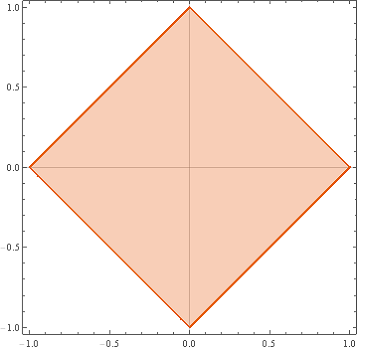
\includegraphics[width=0.4\textwidth]{Norm1.png} 
	        \captionsetup{labelformat=empty}
	        \caption{1. Norm1}
	        \label{fig:Norm1}
	    \end{figure}

		\begin{figure}[h!]
	        \centering
	        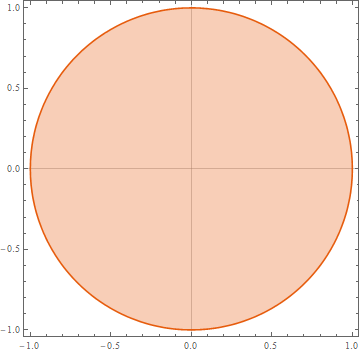
\includegraphics[width=0.4\textwidth]{Norm2.png} 
	        \captionsetup{labelformat=empty}
	        \caption{2. Norm2}
	        \label{fig:Norm2}
	        \end{figure}
	
		\begin{figure}[h!]
	        \centering
	        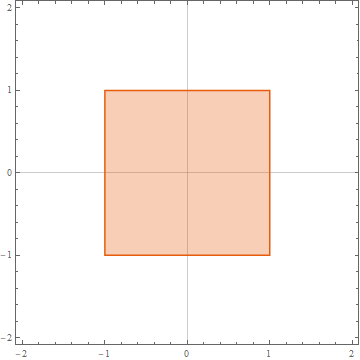
\includegraphics[width=0.4\textwidth]{NormInfinity.png} 
	        \captionsetup{labelformat=empty}
	        \caption{3. Norm Infinity}
	        \label{fig:Norm Infinity}
	        \end{figure}

	\end{soln}

\end{enumerate}




\subsection{Geometry [2 pts]}
Prove the following.  Provide all steps.
\begin{enumerate}
\item 	The smallest Euclidean distance from the origin to some point $\mathbf{x}$ in the hyperplane $\mathbf{w}^\top\mathbf{x} + b = 0$ is $\frac{|b|}{||\mathbf{w}||_2}$.  You may assume $\mathbf{w} \neq 0$.\\
\begin{soln}  
		
		The equation of the shortest euclidean distance from a point to the plane is along the normal to the plane. unit normal vector = $w^{T}/(||w||)$. Shortest distance is the absolute value of the dot product vn (projection on normal vector), where v is the equation of external point to a point on hyperplane, that is,
		$d  = 	(|w^{T}x1 - w^{T}x0|)/||w||  $	
		Putting the value of origin as x0, we get the smallest distance as the above.
 \end{soln}

\item 	The Euclidean distance between two parallel hyperplane $\mathbf{w}^\top\mathbf{x} + b_1 = 0$ and $\mathbf{w}^\top\mathbf{x} + b_2 = 0$ is $\frac{|b_1 - b_2|}{||\mathbf{w}||_2}$ (Hint: you can use the result from the last question to help you prove this one).

\begin{soln}  
		The smallest Euclidean distance from origin to plane1 (as proved above) =  $\frac{|b1|}{||\mathbf{w}||_2}$. Similarly, the smallest Euclidean distance from origin to plane2 =  $\frac{|b2|}{||\mathbf{w}||_2}$.
		Since, the planes are parallel, distance between planes is equal to the difference of smallest distances from origin to each of the planes, that is,   
		\\$\frac{|b2|}{||\mathbf{w}||_2}$ - $\frac{|b1|}{||\mathbf{w}||_2} = \frac{|b2 - b1|}{||\mathbf{w}||_2}.$ 
 \end{soln}

\end{enumerate}



\section{Programming Skills [3 pts]}
Sampling from a distribution.  For each question, submit a scatter plot (you will have 5 plots in total).  Make sure the axes for all plots have the same ranges.
\begin{enumerate}
\item Draw 100 items $\mathbf{x} = [x_1, x_2]^\top$ from a
  2-dimensional Gaussian distribution $N(\mathbf{\mu}, \Sigma)$ with mean $\mathbf{\mu}=(0, 0)^T$ and
  identity covariance matrix $\Sigma=I$, i.e.,
  $p(\mathbf{x}) =
  \frac{1}{2\pi}\exp\left(-\frac{||\mathbf{x}||^2}{2}\right)$, and
  make a scatter plot ($x_1$ vs. $x_2$).  
  
	\begin{soln}
	    
		\begin{figure}[h!]
	        \centering
	        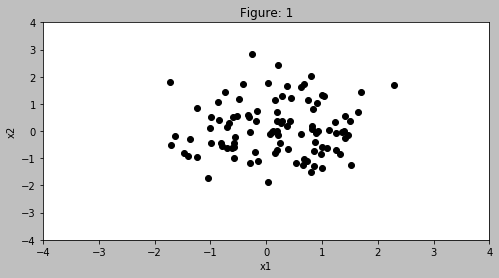
\includegraphics[width=0.6\textwidth]{Assignment_1_Q8_1.png} 
	        \captionsetup{labelformat=empty}
	        \caption{}
	        \label{Fig:1}
	        \end{figure}

	\end{soln}

	\item Make a scatter plot by drawing 100 items from $N(\mathbf{\mu} + (1, -1)^\top, 2 \Sigma)$.
	\begin{soln}
	    
		\begin{figure}[h!]
	        \centering
	        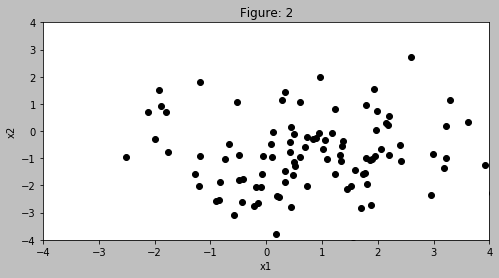
\includegraphics[width=0.6\textwidth]{Assignment_1_Q8_2.png} 
	        \captionsetup{labelformat=empty}
	        \caption{}
	        \label{Fig:2}
	        \end{figure}

	\end{soln}

\item Make a scatter plot by drawing 100 items from a mixture distribution 
$0.3 N\left((1, 0)^\top, \begin{pmatrix} 1 & 0.2 \\ 0.2 & 1\\ \end{pmatrix}\right)
+0.7 N\left((-1, 0)^\top, \begin{pmatrix} 1 & -0.2 \\ -0.2 & 1\\ \end{pmatrix}\right)
$.

  	\begin{soln}
		
		\begin{figure}[h!]
	        \centering
	        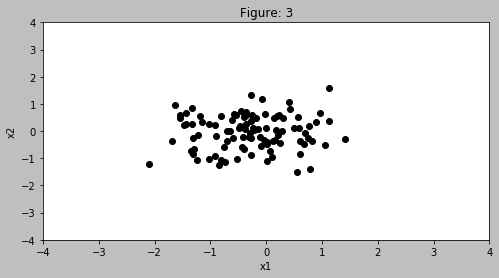
\includegraphics[width=0.6\textwidth]{Assignment_1_Q8_3.png} 
	        \captionsetup{labelformat=empty}
	        \caption{}
	        \label{Fig:3}
	        \end{figure}

	\end{soln}
\end{enumerate}


\bibliographystyle{apalike}


%----------------------------------------------------------------------------------------


\end{document}
